\documentclass[11pt]{article}
\usepackage[margin=1.5in]{geometry}
\usepackage{graphicx}
\usepackage{float}
\usepackage{parskip}
\usepackage{amsmath}
\usepackage{pgfplots}
\pgfplotsset{width=10cm, compat=1.9}

\begin{document}

\textbf{\Huge Introduction to Derivatives}

Athan Zhang \& Jeffrey Chen

\section{The Derivative Function}

\subsection{Definition of the Derivative}
The \textbf{derivative} is one of the fundamental concepts of calculus and is a measure of a function's instantaneous rate of change. The derivative of a function $f(x)$ is written as $\frac{d}{dx}f(x)$ (Leibniz Notation) or $f'(x)$ (Lagrange Notation). The derivative can be interpreted as a function that outputs the slope of the line tangent to $f(x)$ at $x_0$ for any given input point $x_0$ on the domain of $f(x)$.

\begin{center}
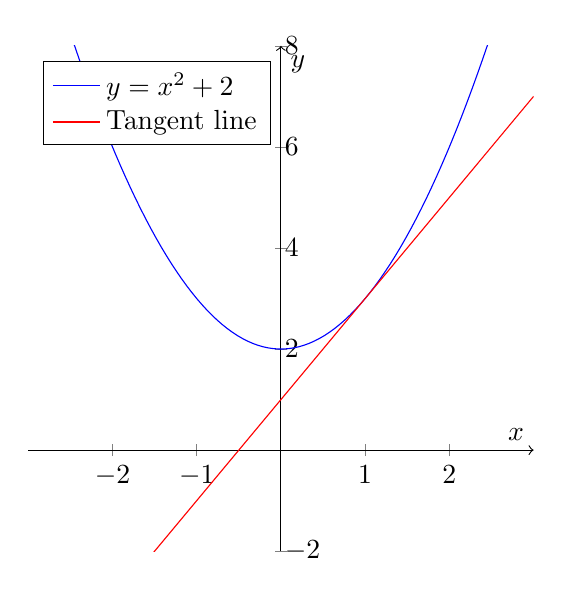
\begin{tikzpicture}
  \begin{axis}[
    xlabel={$x$},
    ylabel={$y$},
    xmin=-3, xmax=3,
    ymin=-2, ymax=8,
    width=8cm, height=8cm,
    axis lines=middle,
    axis line style={->},
    xtick={-2,-1,0,1,2},
    ytick={-2,0,2,4,6,8},
    yticklabel style={anchor=west},
    legend pos=north west,
    legend cell align={left},
  ]

  \addplot[blue, domain=-3:3, samples=100] {x^2 + 2};

  \addplot[red, domain=-3:3, samples=2] {2*x + 1};
  \legend{$y = x^2 + 2$, Tangent line}

  \end{axis}
\end{tikzpicture}
\end{center}

\subsection{Determining the Derivative}
Finding the derivative of a function is commonly known as "taking the derivative." The most basic mathematical definition of the derivative is as follows: given a function $f(x)$ and a secant line passing through $f(x)$ at points $x_0$ and $x_1$, we take the limit of the slope of the secant line as $x_1$ approaches $x_0$:
\[\lim_{x_1 \to x_0} \frac{f(x_1)-f(x_0)}{x_1-x_0}\]
\begin{center}
$\downarrow$
\end{center}
\[f'(x) = \lim_{h \to 0} \frac{f(x_0+h)-f(x_0)}{h}\]
Simple derivatives can be determined using this limit-based definition and formula. However, as our functions of interest become more complex, we desire both simplicity and efficiency in the process of determining derivatives. Therefore, we will introduce \textbf{derivative rules} to help evaluate derivatives much quicker later in this unit.

% problems

\subsection{Higher Order Derivatives}
It is possible, depending on the continuity of the original function $f(x)$, to take the derivative of the function's derivative $f'(x)$. The resulting function, written as $f''(x)$, is known as the second derivative, and so forth. Some functions are infinitely differentiable. This allows us to model certain compound relationships, such as acceleration being the second derivative of position.

% a problem or two 

\section{Basic Derivative Rules}
Derivative rules provide a set of systematic guidelines that allow us to find the derivatives of functions more efficiently. They simplify the process of differentiation by providing a framework to compute derivatives without having to resort to the limit definition every time.

\subsection{Power Rule}
The \textbf{power rule} allows us to easily take the derivative of any power function. It is stated as follows: 

\begin{center}
If $f(x) = x^n$, $n$ being any real number, then $f'(x) = nx^{n-1}$.
\end{center}

\subsubsection{Derivation}

\[f(x) = x^n, f'(x) = \lim_{{h \to 0}} \frac{{f(x + h) - f(x)}}{{h}}\]
\begin{center}
$\downarrow$
\end{center}
\[f'(x) = \lim_{{h \to 0}} \frac{{(x + h)^n - x^n}}{{h}}\]

Expanding \((x + h)^n\) using the binomial theorem, we have:

\[f'(x) = \lim_{{h \to 0}} \frac{{x^n + nx^{n-1}h + \binom{n}{2}x^{n-2}h^2 + \ldots + h^n - x^n}}{{h}}\]
\begin{center}
$\downarrow$
\end{center}
\[f'(x) = \lim_{{h \to 0}} \frac{{nx^{n-1}h + \binom{n}{2}x^{n-2}h^2 + \ldots + h^n}}{{h}}\]

Canceling the common factor of \(h\) in the numerator and denominator, we get:

\[f'(x) = \lim_{{h \to 0}} \left( nx^{n-1} + \binom{n}{2}x^{n-2}h + \ldots + h^{n-1} \right)\]

Taking the limit as \(h\) approaches 0, all the terms with \(h\) vanish except the first term, leaving us with:

\[f'(x) = nx^{n-1}\]


\subsection{Constant Rule}
The \textbf{constant rule} allows us to easily take the derivative of any function scaled by a constant. It is stated as follows: 

\begin{center}
If $f(x) = cg(x)$, $c$ being any real constant scalar, then $f'(x) = cg'(x)$.
\end{center}

\subsubsection{Derivation}
\[f(x) = cg(x), f'(x) = \lim_{{h \to 0}} \frac{{f(x + h) - f(x)}}{{h}}\]
\begin{center}
$\downarrow$
\end{center}
\[f'(x) = \lim_{{h \to 0}} \frac{{cg(x + h) - cg(x)}}{{h}}\]

Applying the distributive property, we have:

\[f'(x) = \lim_{{h \to 0}} \frac{{c (g(x + h) - g(x))}}{{h}}\]

Since \(c\) is a constant, it can be factored out of the limit:

\[f'(x) = c\left(\lim_{{h \to 0}} \frac{{g(x + h) - g(x)}}{{h}}\right)\]

Recognizing that the limit term is the derivative of \(g(x)\), we have:

\[f'(x) = cg'(x)\]

\subsection{Sum Rule}
The \textbf{sum rule} allows us to easily take the derivative of the sum of any two functions. It is stated as follows: 

\begin{center}
If $f(x) = g(x) + k(x)$, then $f'(x) = g'(x) + k'(x)$.
\end{center}
\subsubsection{Derivation}
\[f(x) = g(x) + k(x), f'(x) = \lim_{{h \to 0}} \frac{{f(x + h) - f(x)}}{{h}}\]
\begin{center}
$\downarrow$
\end{center}
\[f'(x) = \lim_{{h \to 0}} \frac{{g(x + h) + k(x + h) - g(x) - k(x)}}{{h}}\]

Applying the properties of limits, we can split the limit into two parts:

\[f'(x) = \lim_{{h \to 0}} \frac{{g(x + h) - g(x)}}{{h}} + \lim_{{h \to 0}} \frac{{k(x + h) - k(x)}}{{h}}\]

Recognizing that the individual limits represent the derivatives of \(g(x)\) and \(k(x)\), respectively, we have:
\[f'(x) = g'(x) + k'(x)\]


\section{Derivatives of Special Functions}
The derivatives of some special non-polynomial functions are useful to derive and memorize as well, due to how often these functions appear. These derivatives should be considered as \textbf{building blocks}, along with the derivative rules introduced in this unit, to solve the derivatives of more complex functions.

\subsection{Trigonometric Functions}
The derivatives of trigonometric functions are a useful tool and should be memorized. They have the property that the derivative of one trig function is comprised of other trig functions. They are as follows:

\begin{table}[H]
    \centering
    \begin{tabular}{|c|c|}
        \hline
        $f(x)$ & $f'(x)$ \\
        \hline
        $\sin{(x)}$ & $\cos{(x)}$ \\ 
        $\cos{(x)}$ & $-\sin{(x)}$ \\
        $\tan{(x)}$ & $\sec^{2}{(x)}$ \\
        \hline
    \end{tabular}
\end{table}

For brevity's sake, only the derivation of the sine function is shown below. Cosine is derived using the exact same method, only swapping respective trig identities. However, the derivation of the tangent function is a bit trickier. It is done using a combination of the sine and cosine derivatives and the quotient rule, which will be discussed later. 

\subsubsection{Derivation of Sine}
\[f(x) = \sin(x), f'(x) = \lim_{{h \to 0}} \frac{{f(x + h) - f(x)}}{{h}}\]
\begin{center}
$\downarrow$
\end{center}
\[f'(x) = \lim_{{h \to 0}} \frac{{\sin(x + h) - \sin(x)}}{{h}}\]

Applying the angle addition formula for sine, we have:

\[f'(x) = \lim_{{h \to 0}} \frac{{\sin(x)\cos(h) + \cos(x)\sin(h) - \sin(x)}}{{h}}\]

Simplifying the expression, we obtain:

\[f'(x) = \lim_{{h \to 0}} \frac{{\sin(x)(\cos(h) - 1) + \cos(x)\sin(h)}}{{h}}\]

Using the trigonometric identity \(\cos(h) - 1 = -2\sin^2\left(\frac{h}{2}\right)\), we can rewrite the expression as:

\[f'(x) = \lim_{{h \to 0}} \frac{{\sin(x)(-2\sin^2\left(\frac{h}{2}\right)) + \cos(x)\sin(h)}}{{h}}\]

Further simplifying, we have:

\[f'(x) = \lim_{{h \to 0}} \left[\sin(x) \cdot \frac{{-2\sin^2\left(\frac{h}{2}\right)}}{{h}} + \cos(x) \cdot \frac{{\sin(h)}}{{h}}\right]\]

Taking the limit as \(h\) approaches 0, we have:

\[f'(x) = \sin(x) \cdot \lim_{{h \to 0}} \frac{{-2\sin^2\left(\frac{h}{2}\right)}}{{h}} + \cos(x) \cdot \lim_{{h \to 0}} \frac{{\sin(h)}}{{h}}\]

Using  limit properties, we know that 
\(\lim_{{h \to 0}} \frac{{\sin(h)}}{{h}} = 1\), and \(\lim_{{h \to 0}} \frac{{-2\sin^2\left(\frac{h}{2}\right)}}{{h}} = 0\)

Therefore, we have:

\[f'(x) = \sin(x) \cdot 0 + \cos(x) \cdot 1\]

Simplifying the expression, we obtain:

\[f'(x) = \cos(x)\]


\subsection{Logarithmic Functions}
The derivative of the logarithmic function is as follows: 

\begin{center}
If $f(x) = \ln(x)$, then $f'(x) = \frac{1}{x}$.
\end{center}

There is no meaningful derivation that can be shown about this property without diving into the origins of $e$ and the natural logarithm. For now, students must be satisfied with this: by the definition of the natural logarithm, its derivative is $\frac{1}{x}$.

\subsection{Exponential Functions}
The derivative of the exponential function is as follows:

\begin{center}
If $f(x) = e^x$, then $f'(x) = e^x$.
\end{center}

\subsubsection{Derivation}
We start with the identity: 

\[ \ln(e^x) = x \]

Next, we differentiate both sides:

\[ \frac{d}{dx} \ln(e^x) = \frac{d}{dx} x \]

Perform chain rule (which will be covered in a following section) on the left hand side to obtain:

\[\frac{1}{e^x} \cdot \frac{d}{dx} e^x = 1\]

Finally, multiply each side by $e^x$ to obtain:

\[\frac{d}{dx} e^x = e^x\]

$0$ is not in the range of $e^x$, so this derivation holds true for all $x$.





\section{Product and Quotient Rules}
\subsection{Product Rule}
The \textbf{product rule} allows us to easily take the derivative of the product of any two functions. It is stated as follows: 

\begin{center}
If $f(x) = g(x) \cdot k(x)$, then $f'(x) = g'(x)k(x) + g(x)k'(x)$.
\end{center}

\subsubsection{Derivation}

\[f(x) = g(x) \cdot k(x), f'(x) = \lim_{{h \to 0}} \frac{{f(x + h) - f(x)}}{{h}}\]
\begin{center}
$\downarrow$
\end{center}
\[f'(x) = \lim_{{h \to 0}} \frac{{g(x + h) \cdot k(x + h) - g(x) \cdot k(x)}}{{h}}\]

Adding an intermediary term, we have:

\[f'(x) = \lim_{{h \to 0}} \frac{{g(x + h) \cdot k(x + h) - g(x + h) \cdot k(x) + g(x + h) \cdot k(x) - g(x) \cdot k(x)}}{{h}}\]

Applying the properties of limits, we can split the limit into two parts:

\[ f'(x) = \lim_{{h \to 0}} g(x + h) (\frac{k(x + h) - k(x)}{h}) + \lim_{{h \to 0}} k(x) (\frac{g(x + h) - g(x) }{h})\]
\begin{center}
$\downarrow$
\end{center}
\[ f'(x) = g(x) \lim_{{h \to 0}}\frac{k(x + h) - k(x)}{h} + k(x) \lim_{{h \to 0}}\frac{g(x + h) - g(x) }{h}\]

Recognizing that the individual limits represent the derivatives of \(k(x)\) and \(g(x)\), respectively, we have:

\[f'(x) = g(x) \cdot k'(x) + k(x) \cdot g'(x)\]

We rearrange to obtain:

\[f'(x) = g'(x)k(x) + g(x)k'(x)\]


\subsection{Quotient Rule}
The \textbf{quotient rule} allows us to easily take the derivative of the quotient of any two functions. It is stated as follows: 

\begin{center}
If $f(x) = \frac{g(x)}{k(x)}$, then $f'(x) = \frac{g'(x)k(x)-g(x)k'(x)}{k^2(x)}$.
\end{center}

\subsubsection{Derivation}
\[f(x) = \frac{g(x)}{k(x)}, f'(x) = \lim_{{h \to 0}} \frac{{f(x + h) - f(x)}}{{h}}\]
\begin{center}
$\downarrow$
\end{center}
\[f'(x) = \lim_{{h \to 0}} \frac{\frac{g(x+h)}{k(x+h)}-\frac{g(x)}{k(x)}}{{h}}\]

Multiplying the whole fraction by $\frac{k(x+h)k(x)}{k(x+h)k(x)}$, we get:

\[f'(x) = \lim_{{h \to 0}} \frac{g(x+h) \cdot k(x) - g(x) \cdot k(x+h)}{(h)(k(x+h))(k(x))}\]

Using limit properties, we can extract factors from the denominator:

\[f'(x) = \lim_{{h \to 0}} \frac{g(x+h) \cdot k(x) - g(x) \cdot k(x+h)}{h} \cdot \lim_{{h \to 0}} \frac{1}{(k(x+h))(k(x))}   \]

We simplify the right hand limit term while adding intermediary terms to the left hand limit to get:

\[f'(x) = \lim_{{h \to 0}} \frac{g(x+h) \cdot k(x) - g(x) \cdot k(x) + g(x) \cdot k(x) - g(x) \cdot k(x+h)}{h} \cdot \frac{1}{k^2(x)}   \]

Next, we use limit properties to separate the limit term into two:

\[f'(x) = (\lim_{{h \to 0}} k(x) \frac{g(x+h)-g(x)}{h} - \lim_{{h \to 0}} g(x) \frac{k(x+h)-k(x)}{h}) \cdot \frac{1}{k^2(x)} \]
\begin{center}
$\downarrow$
\end{center}
\[f'(x) =( k(x)(\lim_{{h \to 0}} \frac{g(x+h)-g(x)}{h}) - g(x)(\lim_{{h \to 0}} \frac{k(x+h)-k(x)}{h})) \cdot \frac{1}{k^2(x)} \]

Recognizing that the individual limits represent the derivatives of \(g(x)\) and \(k(x)\), respectively, we have:

\[ f'(x) = \frac{k(x)\cdot g'(x) - g(x) \cdot k'(x)}{k^2(x)} \]

We rearrange to obtain:

\[ f'(x) = \frac{g'(x)k(x)-g(x)k'(x)}{k^2(x)} \]




\section{Chain Rule}
The chain rule is the final building block required to complete our derivative skills. Mastery over the chain rule allows us to theoretically take the derivative of essentially all functions necessary for this course and even courses beyond. Its usefulness truly has no end. 

The chain rule is a rule that essentially allows us to take derivatives of the composition of two functions. There are many ways of expressing it, the most popular of which is written as: 

\begin{center}
$\frac{dy}{dx} = \frac{dy}{du} \frac{du}{dx}$
\end{center}

However, in my experience, I have found the chain rule to be much easier to understand when expressed in terms of the composition of two functions, as shown below:

\begin{center}
$\frac{d}{dx}f(g(x) = f'(g(x)) \cdot g'(x)$
\end{center}

Both expressions of the rule mean the same thing: by introducing an intermediary function, we can split a complex derivative into the product of two simpler ones. 

\subsection{Derivation}
There are many proofs of the chain rule, involving limits, error functions, and more, but they will not be shown in these notes for the sake of brevity. Any number of proofs can be found online. Instead, take a more intuitive approach to understanding it: when looking at the traditional method of expressing the chain rule, for example, it can be seen that in the product $\frac{dy}{du} \frac{du}{dx}$, the $du$'s cancel each other out, resulting in $\frac{dy}{dx}$. It is much more helpful to understand why this is true than to try and understand a whole rigorous proof of the chain rule.

\subsection{Example}
It is easier shown than explained, so below is an example:

\begin{center}
$ f(x) = sin(e^x) $
\end{center}

\subsubsection{Traditional Expression}
The chain rule process for this example will be explained in terms of both expressions. First off, the traditional expression: we introduce an intermediary function $u(x)$, $e^x$ in this case. Next, we evaluate $\frac{dy}{du}$. $du$ being on the bottom means we take $u(x)$ as our independent variable: 

\begin{center}
$ f(x) = sin(e^x) = sin(u(x)) $\\
$\downarrow$\\
$\frac{d}{du} f(x) = cos(u(x)) = cos(e^x)$
\end{center}

Next, we evaluate $\frac{du}{dx}$: 

\begin{center}
$ u(x) = e^x $\\
$\downarrow$\\
$\frac{du}{dx} = e^x$
\end{center}

Finally, we multiply these two simpler derivatives to obtain our answer:

\begin{center}
$\frac{dy}{dx} = \frac{dy}{du} \frac{du}{dx}$\\ 
$\downarrow$\\
$\frac{dy}{dx} = cos(e^x) \cdot e^x = e^xcos(e^x)$
\end{center}

\subsubsection{Composition Expression}
Next, the example will be explained in terms of the composition-based expression (the more intuitive one, in my opinion). First off, it can be seen that $f(x)$ can be interpreted as the composition of two functions: $sin(x)$ and $e^x$. 

Having noted this, we will take the derivative of the outer function in the composition ($sin(x)$), and keep the inner function ($e^x$) as the input. Essentially:

\begin{center}
$\frac{d}{dx}sin(x) = cos(x)$\\
replace input with inner function\\
$\downarrow$\\
$cos(e^x)$
\end{center}

Next, we will take the derivative of the inner function:

\begin{center}
$\frac{d}{dx} e^x = e^x$
\end{center}

And finally, we multiply the two results to obtain our final answer:

\begin{center}
$\frac{dy}{dx} = cos(e^x) \cdot e^x = e^xcos(e^x)$
\end{center}

% problems

\section{Conclusion}
In conclusion, these rules constitute our metaphorical toolbelt for taking the derivative of any given function. Derivatives have importance in many contextual and analytical applications, many of which will be covered later in this course, but first students must grasp and master the art of calculating them. 

\end{document}
